\chapter[Accounting for haplotype uncertainty in QTL mapping of multiparental populations using multiple imputation]{Accounting for haplotype uncertainty in QTL mapping of multiparental populations using multiple imputation
\footnote{This chapter represents a mature draft of a manuscript currently in preparation, with slight modifications made for the format. Current author line and title are: Keele, G.R., Valdar, W. Accounting for haplotype uncertainty in QTL mapping of multiparental populations using multiple imputation.}}
\label{chap:mi}

\section{Introduction}

Genetic association studies have been extraordinarily successful at identifying genes and regions of the genome that are important to the underlying biological mechanisms modulating complex phenotypes that are highly relevant to medicine and agriculture. Within the context of human studies, genome-wide association studies (GWAS) have been prolific in their ability to identify common variants as candidates for further study \citep{Lee2016}. However, such studies are constrained by their observational nature, complex population structure, and potentially unobserved confounding factors. These challenges, along with constraints in the phenotypes that can be reasonably measured in humans, provide support for controlled experiments in model organism systems, both as models of complex human phenotypes and diseases, as well as agriculturally relevant traits.

% Multiparental populations
Many traditional experimental designs for model organisms result in individuals descended from two founders, or bi-parental populations. These populations have been highly fruitful for QTL mapping, and thus many statistical methodologies have been developed \citep{Broman2001}. A limitation of these simpler populations is that they do not possess as much genetic variation as is in naturally occurring ones, thus limiting their ability to model humans adequately for certain biological systems. Addressing this limitation of bi-parental populations, multiparental populations (MPP) possess greater phenotypic and genetic diversity through the incorporation of additional founders, while often maintaining reproducibility. MPP populations have been developed in a number of species, such as the Collaborative Cross (CC) \citep{Hall2012,Srivastava2017} and Diversity Outbred (DO) stock \citep{Churchill2012} in laboratory mouse; the \textit{Drosophila} synthetic population resource (DSPR) in flies \citep{King2012a, Long2014, King2017, Najarro2017, Stanley2017}; round worm \citep{Noble2017}; yeast \citep{Cubillos2017}; multi-parent advanced generation inter-cross lines (MAGIC) in \textit{Arabidopsis} \citep{Kover2009, Huang2011} and rice \citep{Bandillo2013, Raghavan2017}; nested association mapping population (NAM) in maize \citep{Buckler2009} and sorghum \citep{Bouchet2017}; strawberry \citep{Mangandi2017}; and oil palm \citep{Tisne2017}. The well-characterized founder haplotypes allows for QTL mapping approaches that, rather than modeling phenotype in terms of genotyped variants,  models phenotype with haplotype descent. This haplotype approach allows un-genotyped loci to be tested as putative QTL positions. Although haplotype association will not necessarily outperform genotype association, particularly if a genotyped variant, such as a single nucleotide polymorphism (SNP), is causal or strongly tags the causal variant, it will implicitly model all local variants, possibly including local epistatic interactions specific to a haplotype block that would be challenging to model in a principled way through genotypes. Haplotype association does, however, complicate the statistical methodology due to the fact that haplotypes are not directly observed, but rather probabilistically inferred.

% Haplotype uncertainty
This uncertainty surrounding haplotype, or more generally, genetic state, is formally addressed with interval mapping (IM) \citep{Lander1989}. IM models the data as a mixture of normal distributions, a result of the genetic state uncertainty at an interval or position in the genome, and fits maximum likelihood estimates (MLE) of parameters through an Expectation-Maximization (EM) algorithm \citep{Dempster1977} for Frequentist inference. Genetic state probabilities are estimated for intervals that span the entire genome, either as pseudomarkers (often regularly spaced) or at the genotyped marker positions \citep{Lander1987}. There are a number of Hidden Markov models (HMM) that can be used to construct the probabilistic reconstructions of genetic state, allowing for the incorporation of multiple sources of information and uncertainty, such as genotyping error \citep{Mott2000,Liu2010,Fu2012,Zheng2015} or even incorporate information from genotype probe intensities \citep{Gatti2014}. Although IM was initially proposed in bi-parental populations, first in backcrosses (BC) \citep{Lander1989} and extended for F2 intercrosses and other designs \citep{Dupuis1999}, it has also been generalized to multi-allelic settings \citep{Liu2000a}, such as in MPP. Though IM models the uncertainty in haplotype, in cases of low information distinguishing genetic states, it can become unstable. This issue can be compounded in MPP where there are more genetic states to distinguish at a locus. It is also possible that the EM procedure will become stuck in local maxima, which is also more challenging in MPP where the likelihood is more complex and  multi-dimensional. Finally, the EM is an iterative method, and thus potentially computationally intensive, particularly for dense scans in populations with fine mapping resolution.

%%%%% ROP
The problems of stability and computational efficiency of IM were addressed with an approximate regression approach, sometimes referred to as Haley-Knott regression, though which we will refer to as regression on probabilities (ROP) \citep{Haley1992,Martinez1992}, that involves regressing the phenotype directly on the genetic state probabilities, or some function of the probabilities, such as the additive dosages of an allele. By dosage, we mean a probabilistic generalization of a count of alleles. ROP, also referred to has Haley-Knott regression, was initially proposed for bi-parental populations in which there are only two founder haplotypes, similar to bi-allelic SNPs, and has been extended to multi-allelic populations \citep{Rebai1993}, and is commonly used \citep{Mott2000, Valdar2006a, Valdar2009, Kover2009, Svenson2012, Gatti2014}. Although ROP does not directly model the uncertainty present in the genetic state, the expectations of the modeled data are equivalent in certain settings from the mixture of normals model (IM) and the standard ROP regression. Although it has been known that ROP can produce unstable allele effect estimates \citep{Zhang2014}, it has thus far been considered reliable for hypothesis testing.

% ROP with SNPs
ROP-like approximations have commonly been used in human GWAS, in which it is common practice to use SNP probabilities or dosages for unobserved variants based on probabilistic reconstructions from densely genotyped reference samples (like HapMap \citep{Gibbs2003}). A very simplistic approach is to take the most likely genotype and completely ignore the uncertainty present in the genotype, although ROP procedures have been found to outperform such an approach \citep{Li2009, Aulchenko2010, Marchini2010, Zheng2011}. Though an improvement over completely ignoring uncertainty in the genotypes, ROP does not directly model it and \cite{Kutalik2011} notes that this can lead to an increased false positive rate (FPR) in SNP-based GWAS. This increased FPR is the result of small probabilities correlating strongly with the phenotype, which the ROP procedure will not treat as highly unlikely SNP alleles, but rather as a small SNP dosage that strongly predicts phenotype, resulting in an entirely artificial association. In response to these problems that can occur with the ROP approach, there have been proposed statistical methods, primarily for SNP-based analysis, to directly model the uncertainty \citep{Kutalik2011, Acar2013}, which are similar to IM in model organisms, through the use of an EM procedure. 

% ROP in MPP
This problem of observed false positives resulting from low probability alleles is more avoidable in SNP association than haplotype association, in which it is common practice to filter out SNPs with very low minor allele frequencies (MAF), which are considered likely genotyping errors. This filtering step will also most likely remove the markers that are prone to ROP significance inflation. However, in the multi-allelic setting of MPP, depending on the allelic balance of the population, almost all loci may possess alleles with low allele frequencies, and are thus prone to producing an artificial ROP signal. One approach to countering this issue is to fit the haplotype effects as random effects with a single variance component, thus harnessing shrinkage \citep{Verbyla2014, Wei2016}. Though it is computationally more intensive to fit the QTL effect as a random effect, possibly prohibitively slow in certain data sets and particularly in the presence of population substructure, this approach is preferable to fixed effects. However, fitting the QTL effect as a random term through ROP does not directly address the underlying issue of potential correlations between outcome and probabilities or dosages, but does happen to greatly restrict the problem by dynamically shrinking the potential effects. As such, statistical approaches that more directly model the uncertain nature of inferred genetic state are needed.

%%%%% Bayesian methods
Bayesian approaches offer alternatives to Frequentist QTL mapping methods, and with advances in computing, are becoming increasingly appealing due to their ability to fit complex, highly parametric models, including stably fitting multi-locus models with shrinkage, handling multiple outcome models, and naturally incorporating additional sources of uncertainty through the hierarchical model. Genomic prediction is a natural application of Bayesian models to genetic data due to its focus on optimally fitting and predicting data, thus harnessing the potential of Bayesian statistics for stable yet highly parametric models, such as potentially including all loci \citep{Meuwissen2001, Xu2003, Yi2008}. These ideas can also extend to Bayesian QTL mapping, particularly a fully multilocus approach \citep{Crawford2015}. Here we instead focus on the Bayesian modeling of the genetic state uncertainty jointly with other model parameters in the context of populations descended from inbred founders, allowing this uncertainty to be directly modeled rather than approximated as in ROP. 

A fully Bayesian approach would include genetic state as an unobserved variable in the hierarchical model, allowing the genetic state probabilities to be updated through sampling in response to the other parameters in the model, particularly phenotype and QTL effects. For normal data, often the hierarchical model is specified such that the QTL effect is dependent on the noise variance parameter, resulting in conjugate priors \citep{Servin2007} and a factorizable posterior, allowing Markov Chain Monte Carlo (MCMC) sampling to be avoided, which can be prohibitively slow and fail to mix with complicated models. 

% Sen & Churchill
\cite{Sen2001} propose a comprehensive and generalizable Bayesian hierarchical model for QTL mapping that simultaneously models multiple loci based on a pre-specified grid of pseudomarker locations. A binary vector of QTL status is sampled, and its posterior used for hypothesis testing. To avoid MCMC and still acknowledge that the phenotype can inform the estimate of genetic state, they use an importance sampling scheme with weights calculated based on how well the genetic states at the QTL explain the phenotype, in essence updating the genetic state probabilities, and allowing weighted Monte Carlo (MC) sampling from initial joint multipoint imputations of the genetic states across the pseudomarker grid. Though the model is broadly proposed, it is applied in simpler bi-parental populations assumed to have no population structure. Generalizing the method to MPP is possible, likely requiring the inclusion of a polygenic effect with corresponding variance component as well as imposing shrinkage on QTL effects with variance components. This additional model complexity would likely require MCMC sampling that include computationally expensive matrix operations, and would thus likely be infeasible without further assumptions or approximations.

% Durrant & Mott
A Bayesian mapping approach could be simplified to a single locus perspective, and potentially allow for computationally feasible mapping in MPP. \cite{Durrant2010} proposed a single locus Bayesian QTL mapping approach for MPP that has some similarities to \cite{Sen2001}, such using the conjugate prior for QTL effects as dependent on the noise variance. They also make the assumption that genetic state is independent of phenotype and QTL effect, thus not require updating of the genetic state probabilities and allowing MC sampling. This assumption should be conservative, and greatly reduces the computational burden through the avoidance of MCMC. Notably an important contribution is made through the inclusion of a variance component on the effect of a single locus, imposing shrinkage, and potentially crucial for the more complicated genetic models that result from MPP haplotype alleles. Their method still does not generalize in a computationally feasible way to an MPP with population structure. An additional variance component corresponding to overall relatedness would require either MCMC sampling, which would likely mix poorly and require matrix operations, or a more challenging and extensive MC sampling from the joint non-standard distribution of the variance components.

% Diploffect
Features from the previous methods are shared with other Bayesian models of MPP data. \citep{Zhang2014} proposed the Diploffect model for estimating MPP haplotype allele effects at a locus while taking into account the haplotype uncertainty. Similar to \cite{Durrant2010} its focus is a single locus model for an MPP population; however, it allows for the genetic state parameters to be updated from information in the phenotype and QTL effect through importance sampling, as in \cite{Sen2001}. Briefly, Diploffect is more flexible to modeling of population structure when implemented through integrated nested Laplace approximation, but is not feasible nor intended for a QTL scan across the genome.

% Transition to multiple imputation
The previously described Bayesian methods demonstrate how Bayesian statistics can naturally model and account for many levels of uncertainty. However, they also reflect the computational burden of increasingly complicated genetic models, particularly within a genome-wide context. Though jointly modeling uncertainty on genetic state and parameters would be ideal, incorporating the sampling process on the genetic states with traditional Frequentist likelihood-based inference could account for the genetic state uncertainty and be computationally feasible. In terms of the described Bayesian methods, if the locus effect is fit as a random effect, this would represent a multiple imputation Frequentist version of \cite{Durrant2010}, in which the genetic state probabilities are not updated; essentially the prior is being treated like a posterior and averaged over in the multiple imputation process. And though sacrificing the ability to propagate and characterize the parameter uncertainty that is an important feature of Bayesian statistics, we gain computational efficiency to feasibly model population structure. 

% Describing Frequentist multiple imputation
Although multiple imputation can intuitively be viewed through Bayesian lens as part of the overall sampling process, with each imputation representing a sample from the prior distributions of the missing data, here modeled as parameters in the hierarchical model, inferences can still be drawn using Frequentist methods. This process involves repeating the statistical procedure on each imputed data set, aggregating results, and drawing inference from the summary, therefore incorporating the uncertainty due to missing information, in this case genetic state uncertainty. There have been numerous proposed methods for aggregating statistics over imputations \citep{Li1991}. Commonly regression coefficients are averaged, and incorporated into a multiple imputation version of a Wald statistic. This approach would not naturally generalize to fitting the QTL effect as random effect. \cite{Meng1992} propose an aggregate likelihood ratio test, though it would also require a fixed effect QTL model. \cite{Li1991} also propose aggregating over p-values as an approximate approach for drawing inference across imputations, which would generalize whether the QTL was fit as either a random or fixed effect.

% Comment on imputation terminology
It is important to note that in the context of GWAS, the term imputation is commonly used in reference to estimating variant allele probabilities at unobserved loci. These are related concepts, though we are using its original meaning from the missing data statistics field, whereby an imputation is a sample or realization drawn from a data probability distribution. "Imputed" SNP variants in GWAS usually represent a ROP-like analysis, as is common in SNP-based GWAS, though multiple imputation analyses has been used with SNP data \citep{Ramstein2015}. Here, we propose a multiple imputation approach to haplotype association, in which genetic state, in this context, diplotype state, is imputed from estimated diplotype probabilities. 

A multiple imputation with Frequentist inference approach would control false positives that can occur with ROP while also being computationally convenient. Furthermore, regression-based procedures are easily extended to important modeling considerations such as additional covariates and confounders, population substructure, batch effects, as well as alternative parameterizations of the genetic model (\textit{e.g.} additive model). As such, a Frequentist multiple imputation procedure provides a flexible approach that extends many of the appealing features of ROP, while also accounting for genetic state uncertainty. In addition, such an approach remains computationally feasible for a genome-wide procedure in comparison to fully Bayesian approaches.

\section{Statistical Models and Methods}
We will describe various methods for mapping QTL based on testing how well an individual's genetic state at a locus predicts the phenotype with a linear model. First we will briefly describe our framework.

\subsection{General Framework}
Define $y_{i}$ to be the observed phenotype value of an individual. The genetic state for an individual at a locus is encoded in $\bg_{i}$, a $K$-element vector. The number of genetic states $K$ is determined by the number of allele $J$ such that $K = J + \genfrac(){0pt}{2}{J}{2}$. For bi-allelic variants, such as is common with SNPs, $J = 2$ and $K = 3$. For an eight founder MPP, such as the DO, $J = 8$ and $K = 36$, assuming the population includes individuals that are heterozygous at loci. If a population were completely inbred, $K = J$. The statistical procedures we describe and propose use a single locus approach, with a general model of the form
\begin{equation*}
y_{i} = \text{QTL}_{i} + \varepsilon_{i},
\end{equation*}
in which $\text{QTL}_{i} = \bx_{i}^{\text{T}}\bbetaqtl$ represents the additive linear component of the phenotype $y_{i}$ attributable to the modeled locus, $\bx_{i}^{\text{T}} = \bg_{i}^{\text{T}}\bM$ is the $i$th row of the QTL design matrix $\bX$ representing $\bg_{i}$ rotated according to the model matrix $\bM$, and $\varepsilon_{i}$ as the remainder or residual of $y_{i}$ as an un-modeled error term. 

This simple linear model is appealing in its flexibility, such as allowing alternative parameterizations of the QTL term through $\bM$, which maps between the $K$ genetic states and some linear function of them, often with the intent to simplify the genetic model. One commonly used $\bM$, $\bM_{\text{Add}}$ rotates the genetic state probabilities, which include heterozygous pairings of alleles, to the additive allele dosages. With no uncertainty, $\bM_{\text{Add}}$ maps genetic states to counts of the alleles; in the case of MPP, diplotypes to counts of founder haplotypes. In addition, the model can be expanded to incorporate covariates as fixed effects, as well as split $\varepsilon_{i}$ into multiple components with corresponding variance components, both structured and unstructured. Mapping consists of, for each locus over the genome, testing whether a model with the genetic state at the given locus predicts the modeled phenotype better than a model with no genetic information, or equivalently: 
\begin{equation*}
	H_{0}: \bbetaqtl = \mathbf{0}
\end{equation*}
 When $\bg_{i}$ are directly observed with complete certainty for all $n$ individuals (represented as an $n \times K$ matrix of genetic states $\bG$), this process becomes straightforward. Though these methods could be extended to generalized linear models for non-normal outcomes, we assume that $y$ is a normally distributed trait: 
\begin{equation*}
 	\by | \bG \sim \text{N}(\bX\bbetaqtl, \bV(\btheta))
\end{equation*}
where $\by$ is the $n$-element vector of outcomes, $\bX = \bG\bM$, and $\bV(\btheta)$ is the variance-covariance matrix that includes a parameter vector specifying the variance parameter(s) of the normal distribution. Fitting complex $\bV(\btheta)$ can become computationally prohibitive. There are established approaches to fitting $\bV(\btheta) = \bK\theta_{1} + \bW^{-1}\theta_{2}$, such that $\bK$ is a symmetric relationship matrix and $\bW$ is a diagonal matrix, often the $\bI$ when individuals are weighted equally. Consider the simple situation in which $y$ are independent, then $\theta_{1} = 0$, $\theta_{2} = \sigma^{2}$, and $y_{i} | \bg_{i} \sim \text{N}(\bx^{\text{T}}_{i}\bbetaqtl, \sigma^{2})$. This is equivalent to standard linear regression in which the phenotype is regressed on a linear function of the genetic state. Maximum likelihood estimators (MLE) of the regression parameters ($\bbetaqtl$, $\sigma^{2}$) can be calculated, and used to conduct hypothesis tests. $\btheta_{1} \neq 0$ is often included to model correlations between $y$, such as when population structure is present, at which point a linear mixed effect model is being fit.

Modeling the outcome in terms of genetic state becomes more challenging when the genetic state is not directly observed and thus not known with complete certainty. This uncertainty can arise in the context of assayed genotypes, due to genotyping errors or no-calls. Genetic state can also represent haplotype descent or un-assayed variants, which are not directly observed, but rather probabilistically reconstructed based on LD in nearby genotyped variants.

\subsection{Incorporating uncertainty in genetic state}
The resulting uncertainty in $\bG$ can be described through a probability distribution function $\pr(\bG)$. Formally acknowledging this uncertainty in the association analysis would involve integrating or averaging the likelihood over $\pr(\bG)$:
\begin{equation*}
	\sum_{\bG}\pr(\by|\bG)\pr(\bG)
\end{equation*} 
Accounting for this additional uncertainty lends itself to Bayesian approaches, which allows for hierarchical models to easily be specified. Although additional sources of uncertainty can be intuitively incorporated in Bayesian procedures, the computational cost can be great, and unfeasible particularly when the model becomes complex and includes multiple variance components. An approximate approach that sidesteps the full sampling process of Bayesian statistics is to marginalize out $\bG$, producing a marginal distribution/likelihood, which will be of the form of a normal mixture distribution, and then use hypothesis testing procedures. 

Hypothesis testing is more challenging due to analytic solutions not existing for the MLE of the mixture distribution likelihoods. Instead they must be estimated using an iterative expectation-maximization algorithm (EM) method, which alternates between updating the parameter MLE conditioned on an estimate of the expected value of $\bG$ ($[\bbetaqtlhat, \widehat{\btheta}]^{(t)} | \tilde{\bG}^{(t-1)}$) then re-estimating the expected value of $\bG$ conditioned on the parameter MLE ($\tilde{\bG}^{(t)} | [\bbetaqtlhat, \widehat{\btheta}]^{(t)}$), with $t$ signifying the $t^{\text{th}}$ iteration. This process is repeated until convergence in the MLE is reached ($[\bbetaqtlhat, \widehat{\btheta}]^{(t)} = [\bbetaqtlhat, \widehat{\btheta}]^{(t-1)}$). This mixture model, marginalized over the genetic state probability space, is the statistical procedure used in standard interval mapping (IM) \citep{Lander1989}. 

Though IM accounts for uncertainty in $\bG$, it does not directly jointly model it along with the phenotype, which can result in issues. IM can be unstable (failing to converge or falling into local maxima) particularly if there is little information (high uncertainty) on $\bG$, which can be more likely in MPP (as $J$, the number of founder alleles, increases). One possible alternative to IM draws from the previously mentioned Bayesian perspective which is to explicitly explore $\pr(\bG)$ through sampling. Sampling will require a more complete definition of $\pr(\bG)$.

\subsection{Modeling and sampling genetic state}

We assume that genetic states of individuals, the rows of $\bG$, are independent of each other, thus $\bg_{1}, \bg_{2}, \ldots, \bg_{n}$ can be sampled independently. Violation of this assumption would occur in populations with some level of population structure, but it should not result in a bias even in populations containing close relatives. An intuitive model for $\pr(\bg_{i})$ is
\begin{equation*}
	\bg_{i} \sim \text{Multinomial}(\text{size}=1, \text{probs}=\bphi_{i})
\end{equation*}
with $\bphi_{i}$ representing the ${K}$-element vector of genotype state probabilities, for which $\sum_{k=1}^{K}\phi_{ik} = 1$. $\bPhi$, an $n \times K$ probability matrix with individual $\bphi$ as rows, can be estimated with an HMM, using the information contained in the LD in a window of markers that surround a locus, as well as incorporating additional sources of noise \citep{Mott2000,Fu2012}. We sample genetic state for loci independently, though a multilocus approach could also possible \citep{Sen2001}, based on sampling directly from the HMM (essentially sampling $\boldsymbol{\mathcal{G}}$, an $n \times K \times P$ tensor, $P$ representing the number of loci). A full Bayesian approach would involve conducting the association procedure on each imputation $s$ to produce an association score statistic, $u^{(s)}$. Inference would then be drawn from the posterior distribution of $u$ over many imputations (many samples $\tilde{\bG}^{(s)}$ from $\bPhi$) or alternatively through an importance sampling weighting scheme to reduce the sampling burden, as done in \cite{Sen2001} for simpler bi-parental populations. Extensively sampling from $\pr(\bG)$ could require prohibitively large numbers of imputations, due to the complex probability space of $\pr(\bG)$ that is a result of both the information content (quantified in $\bphi_{i}$) and the number of genetic states $K$. If the data include a large number of individuals and/or the model includes random effects, the complete Bayesian sampling approach can become unfeasible computationally.

\subsection{Conservative multiple imputation procedure}

To avoid a heavy sampling burden, our method is intentionally conservative and not formally Bayesian, primarily targeted at reducing the risk of false positive QTL signals stemming from uncertainty in genetic state. We do not seek to completely or approximately draw inference from posterior distributions, but rather assess the fragility of the association measured through hypothesis tests that results from the uncertainty around $\bG$. We continue to use the single locus model previously described, now sampling imputations for the $\text{QTL}$ term. The procedure uses the following steps:
\begin{enumerate}
	\item Sample $\tilde{\bG}^{(s)}_{p} \sim \text{Cat}(\Phi_{p})$
	\begin{itemize}
		\item For $i = 1, 2, \ldots, n$: \\ $\tilde{\bg}_{ip}^{(s)} \sim \text{Multinomial}(\text{size}=1, \text{probs} = \bphi_{ip})$ 
	\end{itemize}
	\item Regress $\by$ onto $\tilde{\bX}_{p}^{(s)} = \tilde{\bG}^{(s)}_{p}\bM$ for which $\text{QTL}_{i} = \tilde{\bx}^{\text{T}(s)}_{p} \bbetaqtl$
	\item Conduct statistical association test for the presence of a QTL effect, resulting in statistic $u^{(s)}_{p}$
	\begin{itemize}
		\item Compare $H_{0}$: $\bbetaqtl = \mathbf{0}$ versus $H_{A}$: $\bbetaqtl \neq \mathbf{0}$
		\item The multiple imputations procedure is flexible to different statistical tests of association. An F test can be used when there is just one variance component present. With additional variance components, approximate F tests \citep{Halekoh2014} and likelihood ratio tests (LRT) are options.
	\end{itemize}
	\item Repeat steps 1-3 for $s = 1, 2, \ldots, S$ imputations
	\item Summarize over $S$ $u^{(s)}_{p}$ with an aggregate function: $\text{summary}(\bu_{p}) = \bar{u}_{p}$ to produce score of association across the imputations
	\begin{itemize}
		\item As summary, we use the median ($\bar{u}_{p} = \text{median}(\bu_{p})$).
	\end{itemize}
	\item Repeat steps 1-5 for $p = 1, 2, \ldots, P$ loci
\end{enumerate}

\subsection{Median as aggregate statistic}
There has been substantial work on how to aggregate across imputations in terms of Frequentist inference \citep{Li1991}. Tradition, with respect to Wald statistics and likelihood ratio tests \citep{Meng1992}, aggregate test statistics are estimated from averages of the regression coefficients. This is inconvenient for multiple imputation of genetic state because technically it all the data are observed with some level of uncertainty. If a genetic state is likely unobserved, it becomes like that an imputation of the data will not estimate certain genetic state effects, making it awkward to handle averages based on varying numbers of observations. It also does not easily generalize to fitting the locus effect as a random effect.

\cite{Li1991} does mention an approximate approach of aggregating over p-values. Though such a multiple imputation statistic does not perform as optimally in terms of statistical properties, our goal is a conservative, computationally efficient method that will reduce false positives that result from problematic uncertainty in genetic state. Towards this goal, summarizing over p-values is appealing due to its flexibility over differing underlying statistical models. 

In terms of summaries of p-values, we find that the median has a number of appealing characteristics in comparison to an arithmetic mean. With an odd number of imputations, the median is scale independent, even over non-linear, monotonic transformations. This property removes all questions of which scale of a statistic to summarize over. In addition, the mean is sensitive to extreme values, which would emphasize the need for a more complete Bayesian approach with increased sampling $\pr(\bG)$ or weighting through an importance sampling scheme. Therefore, the median is an intuitive and simple approach that reduces the influence of extreme statistics that result from a particular imputations from $\pr(\bG)$, and thus gives a more stable point summary of the association across multiple imputation. Interval summaries can be estimated as confidence intervals on the median as well, based on the binomial distribution with probability parameter $\pi = 0.5$ \citep{Ott2006}, providing a clear way to characterize as well as visualize the stability of the association over imputations.

\subsection{Assessing genome-wide significance}

Genome-wide statistical significance can be assessed through repeating the procedure on permutations of the data when exchangeability can be reasonably assumed \citep{Doerge1996}. Alternatively, if exchangeability cannot be assumed, there are alternatives that do not require it, such as parametric bootstrap samples from the null model. Maximum statistics from the permutation or bootstrap scans are used to fit an extreme value distribution, which is used to specify significance thresholds \citep{Dudbridge2004,Valdar2006c}.

\subsection{Availability of data and software}

All analyses were conducted using the R statistical programming language \citep{RSoftware2018}. The various modeling approaches described for QTL mapping, in particular ROP and MI, and plotting functions can be performed with the R package miqtl, which we make available through a GitHub repository at \url{https://github.com/gkeele/miqtl}.

\section{Simulations}
\subsection{Simulated populations}

Simulations were performed to evaluate how various MPP mapping procedures performed when the causal QTL was known. We simulated 100 samples or realizations of a panel of 200 recombinant inbred (RI) strains, based on the breeding scheme (20 generations of inbreeding) of the CC, using software as used in \cite{Valdar2006c}. We simulated only two chromosomes per individual: chromosome 1 consists of 101 markers, each equally spaced by 1 centi-Morgan (cM), with a single QTL that explains 10\% of the phenotypic variation in the founders at the 55.5 cM position; chromosome 2 contains 201 markers, each spaced by a single cM, and carries no QTL. Both chromosomes allow us to observe the performance of the methods with and without a signal.

\subsection{Tested mapping procedures} 

We used ROP and MI to analyze the simulated CC data, testing the locus effect as either a fixed effect or a random effect \citep{Wei2016}. There mapping approaches are flexible to other modeling considerations such as population structure and nuisance covariates. This flexibility is an valuable feature for many mapping populations, however, our use of simulated CC, which are approximately exchangeable, allow us to consider and compare the following less flexible methods.

We implemented traditional interval mapping through the EM algorithm, in which the probabilistic nature of the data are formally acknowledged by iteratively marginalizing over the genetic state's probability space. IM requires starting parameter values, and we use two approaches for initializing them. We used ROD coefficients and noise variance estimates, which would never be known in real analyses, as the starting values in what we refer to as the oracleIM. For standard IM, we used the sample variance of $\by$ as the starting value of $\sigmasq$ and set the starting founder haplotype effect parameters at 0. 

Finally, we evaluated a maximally expanded data weighted least squares method that we call complete WLS. \cite{Durrant2010} briefly mention expanded data approaches as an approximate Bayesian approach. Maximally expanded means that the data are expanded from $n$ observations to $n \times K$: $\{\by_{\text{aug}}\}_{i} = y_{i} \times \mathbf{1}_{K \times 1}$. The design matrix is similarly expanded: $\{\mathbf{X}_{\text{aug}}\}_{i} = \bI_{K \times K}\bM$. Finally the weights, $\{\bw_{\text{aug}}\}_{i} = \bphi_{i}$, match the corresponding $K$ genetic states encoded in $\{\bPhi\}_{i}$ and $\{\bX_\text{aug}\}_{i}$. When there is no uncertainty around $\bG$, complete WLS will converge to ROD just as ROP, MI, and IM do, as the $K-1$ false genetic states will be given a weight of zero. Complete WLS has the unappealing characteristic of making the data very large, and thus potentially challenging computationally for large data sets. It also does not generalize in a reasonable way to allow for an additional variance component to account for population structure. We wished to see how it performed in comparison to the other methods in the setting in which these shortcomings are not present. \textbf{Table \ref{tab:mapping_procedures}} summarizes the evaluated methods.

\subsection{Simulation of uncertainty}

We simulated the underlying haplotype states rather than marker genotypes, as these methods in MPP are primarily focused on haplotype-based association. Simulating haplotypes allows us to compare the performance of the methods when there is complete certainty to when there is uncertainty. We use two approaches to sample simulated probabilities from the true genetic states: probability dilution and Dirichlet sampling.

\subsubsection{Probability dilution:} The probability dilution process converts a genetic state vector to a probability vector ($\bg \rightarrow \tilde{\bphi}$) in a deterministic manner. Let $\bg_{i,p}$ be the $K$-element genetic state vector for individual $i$ and locus $p$. The true genetic state, corresponding to a $k=t$ element of $\bg_{i,p}$: $g_{itp} = 1$, and all other elements ($k \neq t$) are 0. We perform probability dilution by setting the probability of the true genetic state, $\alpha$, to some value in $[0, 1]$ and all other elements to $\frac{1 - \alpha}{K - 1}$. Of note, for any specification of $\alpha$, any individuals with the same genetic state vector $\bg$ will also have the same realized probability vector $\tilde{\bphi}$.

From a technical perspective, probability dilution does output probabilities, as they are non-negative and sum to 1. However, as simulations of uncertainty around genetic state, they are unrealistically clean, as a predetermined pattern of uncertainty will perfectly correlate with true genetic state. To break this hard correlation between uncertainty and genetic state, we use Dirichlet draws from the genetic state vector of an individual, which is the reverse process of our multiple imputation procedure.

\subsubsection{Dirichlet sampling:}
As with the probability dilution process, we have simulated individual $i$ with a $K$-element genetic state vector $\bg_{ip}$ for locus $p$. We sample a probability vector according to 
\[
\tilde{\bphi}_{ip}^{(s)} \sim \text{Dirichlet}\left(\tilde{n}\alpha\bg_{ip} + \tilde{n}\frac{(1 - \alpha)}{K-1}(\mathbf{1} - \bg_{ip})\right),
\]
such that $\mathbf{1}$ is a $K$-element vector of 1's, and $\tilde{n}$ is a total number of pseudocounts. Similar to our probability dilution specification, $\alpha$ is used to control the probability mass placed on the true and false genetic states; however, now the process is stochastic and thus described in terms of probabilistic expectations. The expected probability for the true genetic state and the false states follows from the Dirichlet: $\text{E}(\tilde{\phi}_{i}^{\text{true}}) = \alpha$ and $\text{E}(\tilde{\phi}_{i}^{\text{false}}) = \frac{1 - \alpha}{K-1}$. The variance of the true probability states follows: $\text{Var}(\tilde{\phi}_{i}^{\text{true}}) = \frac{\tilde{n}\alpha(\tilde{n} - \tilde{n}\alpha)}{\tilde{n}^{2}(\tilde{n} + 1)}$. We can set the expected uncertainty around the true genetic state to be equivalent to the pattern of uncertainty produced by probability dilution, but allowing for more realistic levels of noise. How far samples deviate from expectation due to the noise can be manipulated with the pseudocount parameter ($\tilde{n}$), with lower values having higher noise and higher values approaching probability dilution. A similar Dirichlet sampling scheme was used for SNP genotypes \citep{Acar2013}, however the the probability is spread more thinly in inbred MPP setting with $K=8$ compared to $K=3$ with bi-allelic SNPs.

It is challenging to simulated probabilistic genetic data as would likely be observed in real data, such as sets of genetic states being less distinguishable at certain loci, which is already known to hamper allele effect estimation \citep{Zhang2014}. Another potential realistic issue is differential levels of uncertainty for individuals in the same dataset, which will not be captured in these simulations. The space of potential patterns of uncertainty that could occur in MPP genetic states makes it effectively impossible to explore all of them in a systematic way. While these probability simulation schemes generally place the most probability mass on the true genetic state, which will generally favor ROP, we can still observe how the various mapping procedures perform with varying specifications of the simulation parameters.

\section{Data Sets}

We include examples from three different data sets that come from different types of MPP populations to demonstrate the differences between MI and ROP associations that can occur in actual data, which can differ strikingly from idealized simulated data.

The first example population is composed of 989 individuals from an outbred rat heterogeneous stock (HS) \citep{SolbergWoods2012,Keele2017}, referred to as HS1. The rats were measured on various diabetes and obesity phenotypes. The second population consists of 1407 individuals from a rat HS, independent from HS1 but derived from the same founder strains, that were measured for a large number of phenotypes, and are described in greater detail in \cite{Baud2013, Baud2014}. This population will be referred to as HS2.

The third population is from the CC. A more thorough description can be found in \cite{Mosedale2017}. Briefly, the experimental design involved treating four male mice from each of 45 CC lines with tolvaptan, a candidate treatment for kidney disease, while another four male mice from each line received vehicle (control) instead. In terms of modeling, CC lines from separate breeding funnels are approximately independent from each other, and thus do not require a random effect and associated genetic relationship matrix to model population structure. However, replicate observations from the same CC line due require special modeling considerations, such as a random effect with independent levels, or regression on strain means \citep{Zou2006}, as was used in \cite{Mosedale2017}. 

We highlight differences between these populations to emphasize the need for statistical mapping procedures that can flexibly accommodate multiple sources of variation. For instance, experiments designed for the CC can have genetic replicates, whereas each HS individual has a unique genome. Although the HS will not contain the strongly structured correlations between individuals as expected from genetic replicates in the CC, the rotational breeding scheme produces more subtle population structure as a result of individuals being differentially related to each other rather than approximately equally related (as in CC lines from independent breeding funnels, like our simulations). ROP and MI are much more accommodating to these features than traditional IM, and for this reason, we used only them for analyses of real populations.

\section{Results}

\subsection{Illustration of false association with ROP}

Before presenting simulation results, we provide an example that demonstrates a need for our MI procedure in real data, in this case the HS1 rat population. In populations with high degrees of genetic state uncertainty and allele frequency imbalance, the genome scans from ROP and MI can strikingly differ, as in \textbf{Figure \ref{fig:Leah_example}} which depicts analyses of serum cholesterol levels in HS1.

A striking characteristic of spurious QTL that occur with ROP is an extremely narrow association peak, depicted in \textbf{Figure \ref{fig:Leah_example}A}, particularly the peak on chromosome 11. Many of these associations completely disappear with MI (\textbf{Figure \ref{fig:Leah_example}E}), suggesting that the associations are completely the result of the ROP approximation. This conclusion is further strengthened by closer inspection of the uncertainty present at the sharp peak on chromosome 11, presented in \textbf{Figure \ref{fig:Leah_example}F}. Notably, the B founder allele is highly unlikely to have been observed in the population at this locus, though is still present in the model due to uncertainty. Ultimately a highly inflated association score is produced due to very small dosages that strongly correlate with the phenotype. MI corrects for these occurrences because these rare alleles are rarely or never observed in the imputations. This inflation in significance can be seen in association studies with SNP dosages; however bi-allelic SNPs can be easily screened for low MAF, whereas many loci, even most in a population with high founder haplotype frequency imbalance, such as an HS, have founder haplotype alleles with very low frequencies.

\begin{figure}
\renewcommand{\familydefault}{\sfdefault}\normalfont
\centering
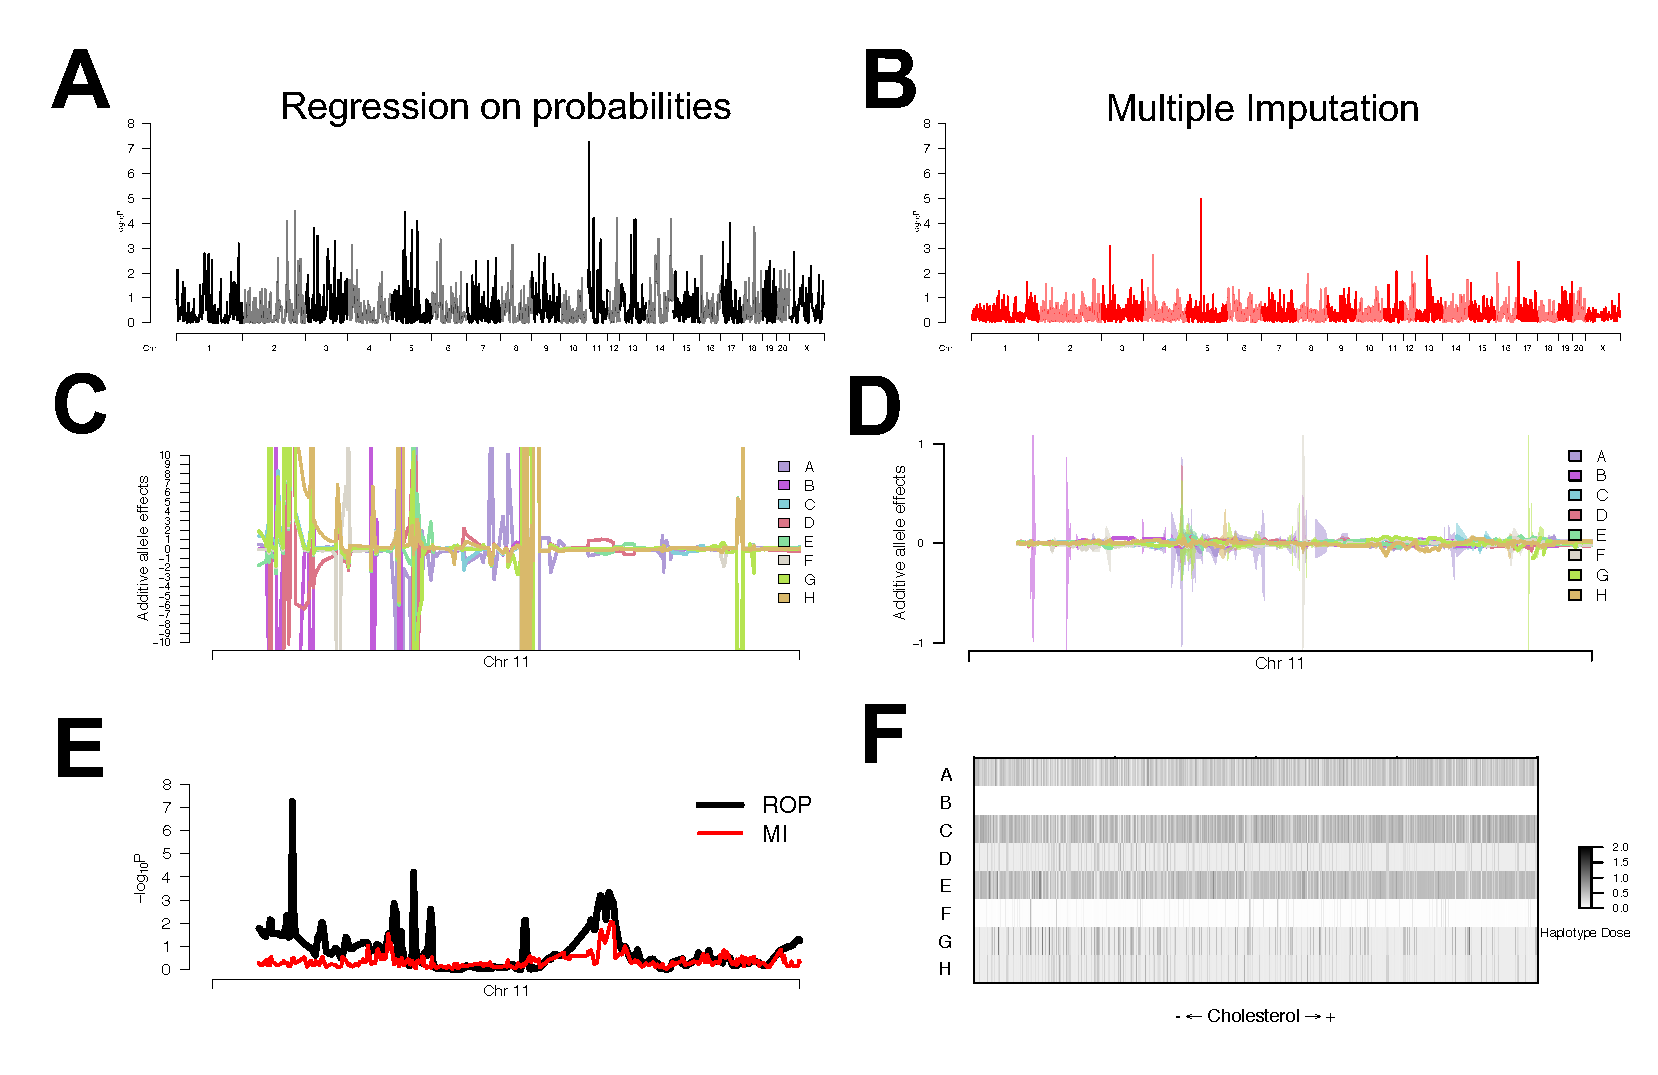
\includegraphics[width=\textwidth]{figures/4-mi/Leah_example.pdf}
\caption[Comparison of ROP and MI in HS rat data]{Analysis of blood cholesterol levels in the HS1 rat population. Genome scans with ROP (A) and MI (B) show drastically different patterns of association. Additive founder haplotype effects, labeled A through H, estimated from regression coefficients for ROP (C) and MI (D), across chromosome 11. The ROP effects are highly unstable, as a result of the highly unbalanced founder haplotype frequencies. For MI effects, transparent color bands represent the 95\% confidence interval for the mean additive haplotype effect over 11 imputations, highlighting regions in which effects are unstable over imputations and in which an allele is unobserved. A comparison of the associations on chromosome 11 reveals that the sharp QTL associations that occur with ROP are almost completely reduced with MI (E). The uncertainty in haplotype dosages observed at the chromosome 11 locus is problematic for ROP and results in inflated associations that are not observed with MI (F). The rows of the probability grid plot represent the haplotypes of the founders. A column of the grid represents the genetic state of a single individual at the a single locus, with the shading of each cell representing the magnitude of haplotype dose. The individuals (columns) are ordered left to right by phenotype rank, allowing for potential haplotype effects to be seen from the raw data, which will appear as cluster in the founder haplotype rows. No clusters are immediately obvious, and more so, the uncertainty present in the dosages is extensive with founders D, G, and H being poorly distinguishable. Additionally there is broad founder allele frequency imbalance, with essentially no haplotype B alleles observed, and very little of the F allele. The strong association is a result of a strong correlation between near-zero probabilities in allele B and the phenotype. \label{fig:Leah_example}}
\end{figure}

\subsection{Simulated results}

Considering the strikingly different genome scans seen in the HS1 data, we assessed the performance of various mapping procedures in simulated MPP data. We simulated 100 realizations of breeding funnels corresponding to the strategy used for the CC, producing a panel of 200 RI strains. We then evaluated the performance of ROP fixef, ROP ranef, MI fixef, MI ranef, IM, oracleIM, and complete WLS (\textbf{Table \ref{tab:mapping_procedures}}) on these simulated populations. We were primarily interested in how the methods responded to increasing level of uncertainty in the genetic state at the simulated QTL as well as at unassociated loci. The genome scan of a single realization of a simulated population, as well as a depiction of the underlying genetic state at the QTL position, when no uncertainty is obscuring genetic state can be seen in \textbf{Figure \ref{fig:sim_truth}}.

\begin{figure}
\centering
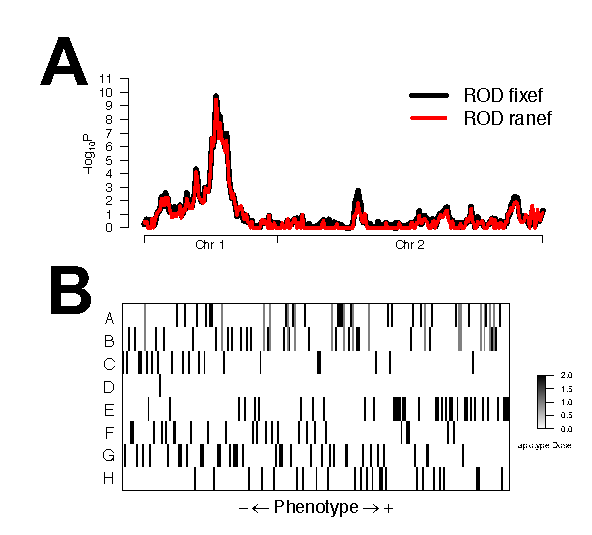
\includegraphics[width=0.6\textwidth]{figures/4-mi/fixef_mapping_truth.pdf}
\caption[Simulated CC-like population with no uncertainty]{The first and second chromosomes of a simulated panel of 200 CC-like RI strains with a single QTL that explains 10\% of phenotypic variance were simulated. The QTL is located on chromosome 1, and no QTL are present on chromosome 2. Association scans of a single simulated population (A). The fixed effect procedure (fixef) and random effect procedure (ranef) generally track similarly, though ranef produces a lower significance score of association due to shrinkage. The simulated haplotype counts represented as an $8 \times 200$ grid, ordered along the x-axis by phenotype (B). A single column of the grid represents the genetic state of an individual at the QTL, with the shading of $i,j$-th cell corresponding to count of haplotype $j$ for individual $i$. As there is no uncertainty of genetic state, all shaded cells represent counts of 0, 1, and 2, which are white, gray, and black respectively. A Non-zero effect is clear in E, and potentially other alleles. The grid gives a clear visual representation of the level of uncertainty at a locus for a given population.\label{fig:sim_truth}}
\end{figure}

\begin{figure}
\renewcommand{\familydefault}{\sfdefault}\normalfont
\centering
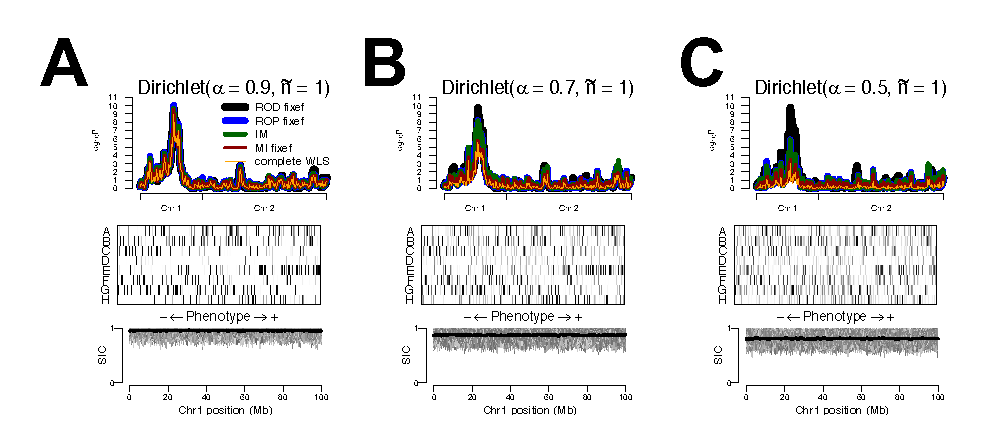
\includegraphics[width=\textwidth]{figures/4-mi/fixef_mapping_uncertainty_dirichlet.pdf}
\caption[Effect of uncertainty modeled through Dirichlet sampling on genome scan in a single simulated CC-like RI panel]{Comparison of mapping approaches with varying levels of Uncertainty in genetic state simulated through Dirichlet sampling with $\alpha = 0.9$ (A), $\alpha = 0.7$ (B), and $\alpha = 0.5$ (C), all with pseudocount $\tilde{n} = 1$ in 200 simulated CC-like RI strains with a QTL that explains 10\% of phenotypic variation on chromosome 1. With Dirichlet sampling, $\alpha$ is the expected probability mass on true genetic state and $\tilde{n}$ determines the variability over Dirichlet samples. For a given $\alpha$, the expected probability vector is equivalent to the probability vector from the probability dilution process, as in Figure \ref{fig:sim_scans_dilution} ($\text{E}(\bphi^{\text{Dirichlet}}_{i, \alpha}) = \bphi^{\text{Dilution}}_{i, \alpha}$). The middle plot of each subfigure depicts the simulated uncertainty at the QTL for the three scenarios. The bottom plot of each subfigure is the the SIC across chromosome 1. Described in greater detail in \cite{Ronnegard2011}, briefly, SIC is a standardized Kullback-Leibler divergence, which we use as a measure of the information content on the genetic state probabilities of an individual ($\bphi_{i}$) at a locus. $\text{SIC} \in [0, 1]$, with the boundaries corresponding to genetic states being completely indistinguishable ($\bphi_{i} = \frac{1}{K} \times \mathbf{1}_{K \times 1}$) and complete certainty ($\bphi_{i} \rightarrow \bg_{i}$), respectively. It is important to note that SIC does not reflect whether the information in the genetic state probabilities are correct. \label{fig:sim_scans_dirichlet}}
\end{figure}

Given a simulated population with known genetic states for all individuals, we then simulated uncertainty in genetic state through either probability dilution or Dirichlet sampling from the vector of true genetic state. 

\subsubsection{Dirichlet sampling:} For a single simulated population, as expected, as the level of uncertainty increases, the association at the QTL is reduced (\textbf{Figure \ref{fig:sim_scans_dilution}}). Complete WLS seems the most penalized by increasing uncertainty, then MI, and finally ROP and IM do the best. We include only the fixed effect models of ROP and MI to both minimize visual clutter and because the fixed effects models are more comparable to IM and complete WLS. In the single simulation, we do not see inflated spurious associations with ROP as seen in real data, though it is important to look across all the simulated data sets. 

Across all simulated data, we see similar trends to the single data set (\textbf{Figure \ref{fig:multi_pval_count1_qtl}}). To assess the mapping procedures across many simulated populations, we evaluated the change in p-value at the QTL and unassociated locus. The associations from ROP and IM degrade the least as uncertainty increases, and MI performs better than complete WLS. At an unassociated locus, all the procedures performed similarly and did not produce false associations. The conservative nature of MI and complete WLS compared to ROP and IM was consistent at the QTL and an unassociated locus.

\subsubsection{Probability dilution:} 
The results for simulations of genetic state uncertainty through probability dilution, a deterministic process, were consistent with Dirichlet sampling, though with a few notable exceptions. For the single simulated population, ROP performs as well as ROD, which can be seen in \textbf{Figure \ref{fig:sim_scans_dilution}}. The performance of IM at the QTL is reduced, but to a lesser extant than seen with Dirichlet sampling, despite the SIC content being lower with dilution, suggesting that the noisier Dirichlet sampling obscures the signal more. MI and complete WLS are both penalized similarly with either Dirichlet sampling or dilution.

Across all 100 simulated populations, we see these same trends. ROP loses none of the statistical signal, except at the point in which each genetic state has the exact same probability (\textbf{Figure \ref{fig:multi_pval_dilution_qtl}}). IM performs better than with Dirichlet sampling, though at the unassociated locus, some false positives occur when uncertainty is very high (\textbf{Figure \ref{fig:multi_pval_dilution_null}}). MI and complete WLS are consistent across Dirichlet sampling and probability dilution, at the QTL and unassociated locus.

The probability grid plots in \textbf{Figures \ref{fig:multi_pval_dilution_qtl}, \ref{fig:multi_pval_dilution_null} [bottom row]} reveal that probability dilution is a very artificial form of uncertainty simulation, as no noise is incorporated to distort the true signal. Thus ROP is able to handle the probabilities as artificial doses that perfectly track with the simulated truth. Similarly, IM handles the uncertainty from probability dilution very well, with only minor reduction in the association at the QTL, though the association does become more unstable across simulations and potentially inflated at the null locus where there is no signal. Likely, this strong performance results from the fact that though IM is probability aware, it is not sampling over the space, but rather iteratively marginalizing over the genetic state space. When no noise is incorporated into the system, as with probability dilution, this marginalization is very effective at capturing the signal. MI involves a full sampling process, and is thus heavily penalized by the greater uncertainty, which it explores despite the signal not being reduced through dilution. Complete WLS is similarly harshly penalized.

We find that Dirichlet sampling of genetic state uncertainty more equally affects all mapping procedures, and more realistically represents realistic patterns of uncertainty. From the probability grids and SIC plots, it is clear that the level of uncertainty is actually lower in the Dirichlet simulations, but that it importantly does not track perfectly with the true genetic state. This leads to ROP and IM being penalized as well, though they still perform better than MI and complete WLS. We also re-emphasize that given an $\alpha$, as $\tilde{n} \rightarrow \infty$, then Dirichlet sampling will converge to probability dilution.

\begin{table}
\renewcommand{\familydefault}{\sfdefault}\normalfont
\begin{minipage}{\textwidth}
%\captionsetup{width=\textwidth}
\centering
\caption[Mapping procedures for simulated data]{Mapping procedures for simulated data (\textbf{Figures \ref{fig:sim_scans_dirichlet}, \ref{fig:multi_pval_count1_qtl}, \ref{fig:multi_pval_count1_null}, \ref{fig:sim_scans_dilution}, \ref{fig:sim_scans_dilution}, \ref{fig:multi_pval_dilution_qtl}, \ref{fig:multi_pval_dilution_null}})
\label{tab:mapping_procedures}}
\end{minipage}

\begin{minipage}{\textwidth}
\begin{tabularx}{\textwidth}{c|c|c|l}
\hline
\makecell{\textbf{Mapping} \\ \textbf{procedure}} 
& \makecell{\textbf{Color} \\ \;} 
& \makecell{\textbf{Uncertainty} \\ \textbf{status}} & \makecell{\textbf{Description} \\ \;} \\
\hline
\makecell{ROD fixef \\ \;} & \cellcolor[HTML]{000000} & \makecell{No uncertainty \\ \;} & \makecell[l]{Regression with complete certainty on genetic \\ \qquad state and locus effect fit as a fixed effect} \\
\hline
ROP fixef & \cellcolor[HTML]{0000FF} & Unaware & ROP with locus effect fit as a fixed effect \\
ROP ranef & \cellcolor[HTML]{87CEEB} & Unaware & ROP with locus effect fit as a random effect \\
\hline
MI fixef & \cellcolor[HTML]{8B0000} & Aware & MI with locus effect fit as a fixed effect \\
MI ranef & \cellcolor[HTML]{FF0080} & Aware & MI with locus effect fit as a random effect \\
\makecell{IM \\ \;} & \cellcolor[HTML]{006400} & \makecell{Aware \\ \;} & \makecell[l]{IM with initial parameter values set to sample \\ \qquad founder means and sample variance} \\
\makecell{oracle IM \\ \;} & \cellcolor[HTML]{00FF00} & \makecell{Aware \\ \;} & \makecell[l]{IM with initial parameters set to ROD fixef \\ \qquad parameter estimates} \\
\makecell{complete WLS \\ \;} & \cellcolor[HTML]{FFA500} & \makecell{Aware \\ \;} & \makecell[l]{Weighted regression with full data expansion \\ \qquad of genetic states} \\
\hline
\end{tabularx}
\end{minipage}
\end{table}


\begin{figure}
\renewcommand{\familydefault}{\sfdefault}\normalfont
\centering
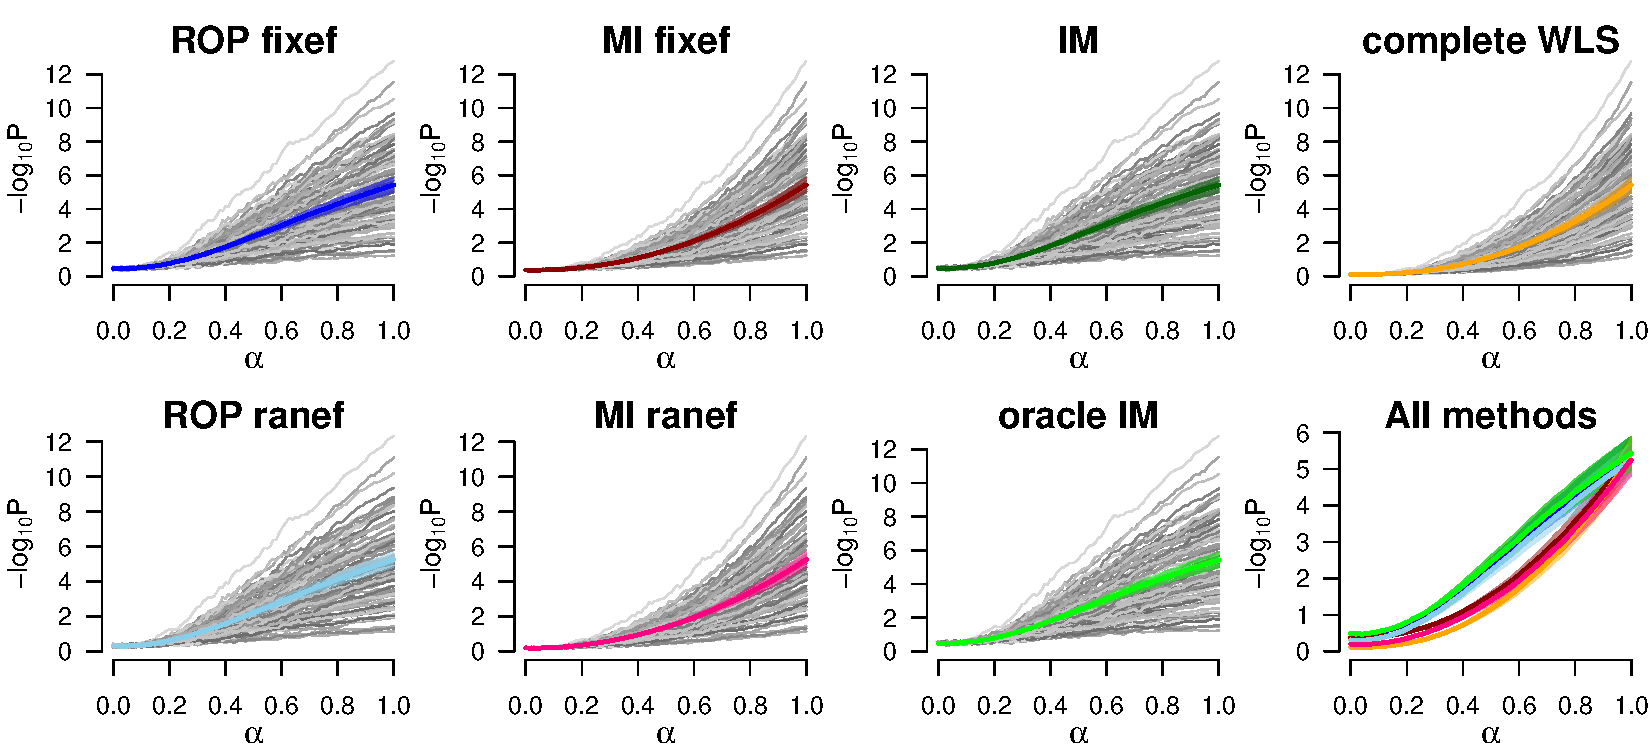
\includegraphics[width=\textwidth]{figures/4-mi/CC_pvalue_fluct_qtl_mean_count1.pdf}
\caption[Effect of uncertainty modeled through Dirichlet sampling on association at QTL in simulated data]{The change in association at 10\% QTL with varying levels of uncertainty, simulated through Dirichlet sampling. $\alpha$ is the expected probability mass of the true genetic state, with the pseudocount parameter ($\tilde{n}$) determining sampling variance. We have set $\tilde{n} = 1$.  Colored lines and transparent bands represent the mean p-value and 95\% confidence interval on the mean p-value for the various mapping procedures (\textbf{Table \ref{tab:mapping_procedures}}) over the 100 populations. Gray lines represent the $-\log_{10}\text{P}$ for a single population. Because the Dirichlet sampling process is random, the gray lines represent mean $-\log_{10}\text{P}$ from 100 Dirichlet sampling steps of the simulated population.\label{fig:multi_pval_count1_qtl}}
\end{figure}

\begin{figure}
\centering
\renewcommand{\familydefault}{\sfdefault}\normalfont
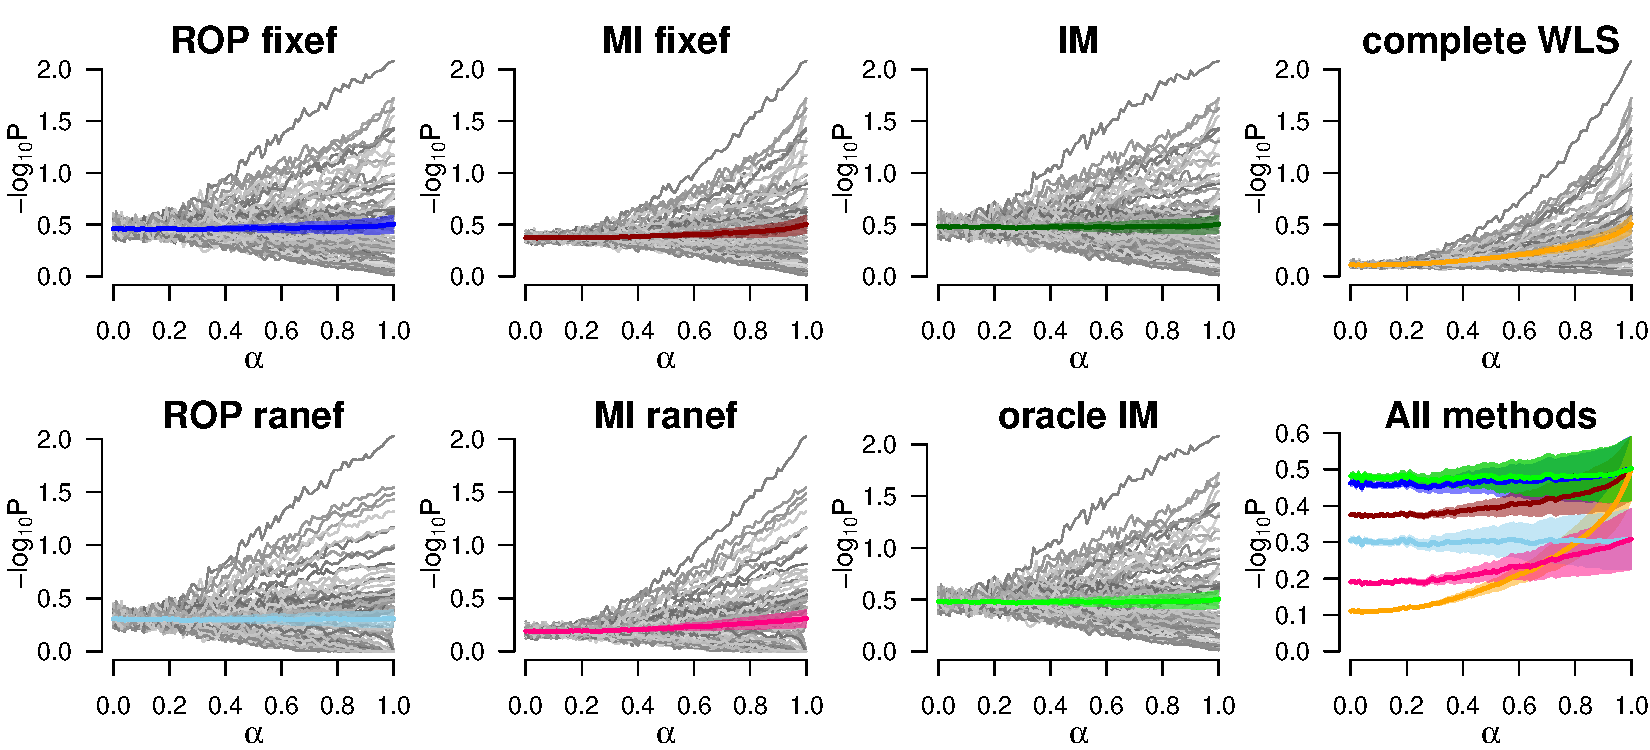
\includegraphics[width=\textwidth]{figures/4-mi/CC_pvalue_fluct_null_mean_count1.pdf}
\caption[Effect of uncertainty modeled through Dirichlet sampling on association at null locus in simulated data]{The change in association at a null locus with varying levels of uncertainty, simulated through Dirichlet sampling. $\alpha$ is the expected probability mass of the true genetic state, with the pseudocount parameter ($\tilde{n}$) determining sampling variance. We have set $\tilde{n} = 1$.  Colored lines and transparent bands represent the mean p-value and 95\% confidence interval on the mean p-value for the various mapping procedures (\textbf{Table \ref{tab:mapping_procedures}}) over the 100 populations. Gray lines represent the $-\log_{10}\text{P}$ for a single population. Because the Dirichlet sampling process is random, the gray lines represent mean $-\log_{10}\text{P}$ from 100 Dirichlet sampling steps of the simulated population.\label{fig:multi_pval_count1_null}}
\end{figure}

\subsection{More examples of results in real populations}

The analyses of simulated data found ROP be an effective approximate approach that performs as well as IM when genetic state uncertainty is realistically simulated through probability dilution. Despite the strong performance of ROP in simulated data, we return to real data to focus on populations with lower levels of genetic state uncertainty and more balanced founder haplotype frequencies compared to HS1 to assess whether ROP could still produce inflated associations in real data that are more similar to the simulated data. In actual CC data, from which the simulated populations were modeled, we still see less extreme examples of the inflated associations (as in HS1) that are reduced though multiple imputation (\textbf{Figure \ref{fig:CC_example}}). In particular, the chromosome 14 peak is stable over multiple imputation, whereas chromosomes 12 and 16 have narrow peaks that are reduced (\textbf{Figure \ref{fig:CC_example}C}). 

\begin{figure}
\renewcommand{\familydefault}{\sfdefault}\normalfont
\centering
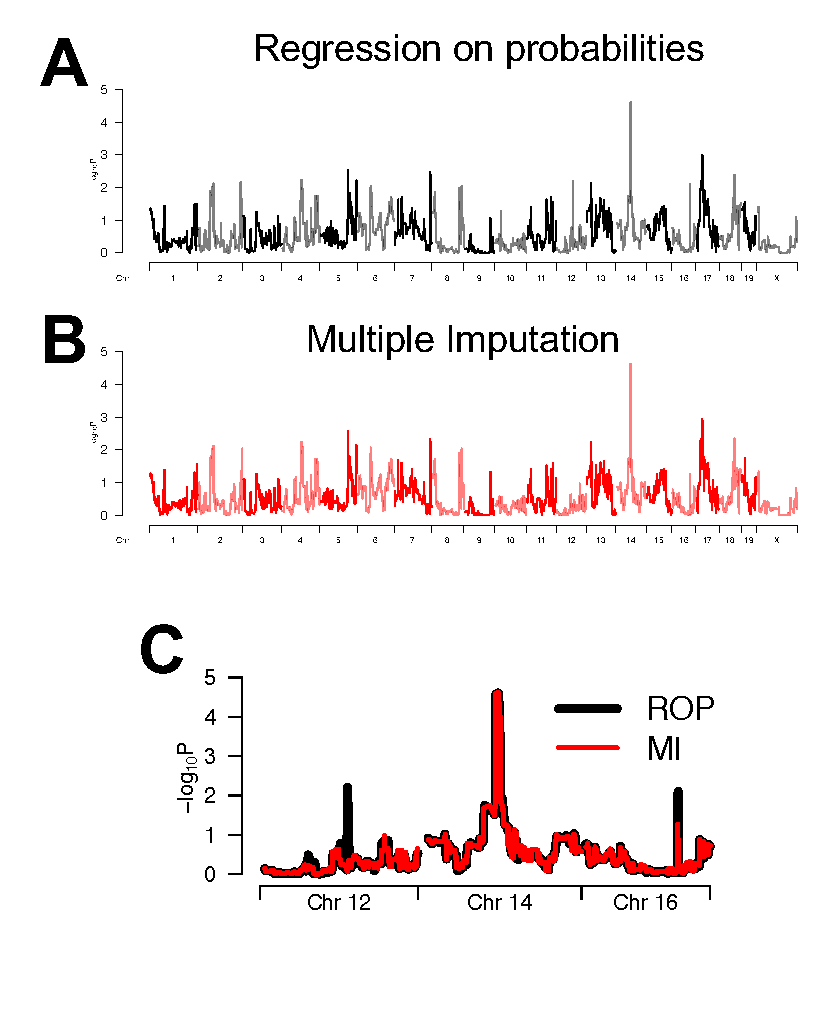
\includegraphics[width=0.8\textwidth, trim={0in 0.5in 0in 0in}, clip]{figures/4-mi/CC_example.pdf}
\caption[Comparison of ROP and MI in CC data]{Example analysis of response to kidney drug in a sample population of 45 CC strains with a total of 159 individuals. Genome scans through ROP (A)and MI (B) show similar associations, though MI lowers some narrow signals. Notable QTL associations for chromosomes 12, 14, and 16 for ROP and MI (C). A notable signal that is consistent across ROP and MI is on chromosome 14. The chromosome 12 and 16 signals are only present with ROP. \label{fig:CC_example}}
\end{figure}

In real CC data, false associations can be inflated beyond what was observed with the clean simulated data. Though more conservative than ROP, MI can reduce these associations while detecting stable associations. The ability of MI to detect QTL is further demonstrated in the larger HS rat population HS2 (\textbf{Figure \ref{fig:AMelie_example}}). The similarity of the genomes scans of HS2 through ROP and MI suggest there is less genetic state uncertainty and founder haplotype imbalance in HS2. With MI the strong associations at chromosomes 4 and 8 are maintained in MI, and are even strengthened compared to the other associations due to the less inflated MI associations. Lesser ROP significant associations on chromosomes 4 and 11 drop below significance with MI. MI also appears to support a peak on chromosome 14 as being near significance compared to its association in ROP. These results show that MI can reliably capture similar associations as ROP, while generally reducing or removing questionable ones.

\begin{figure}
\renewcommand{\familydefault}{\sfdefault}\normalfont
\centering
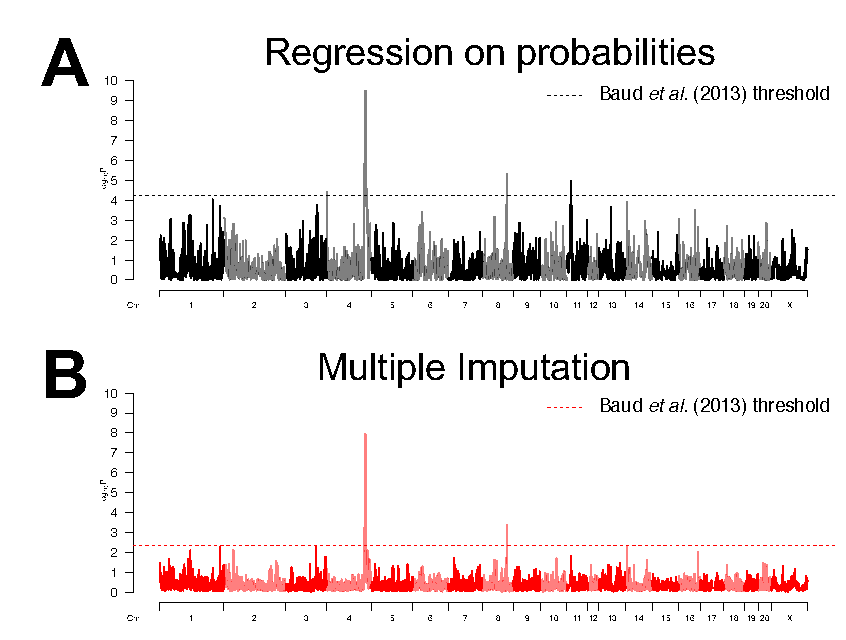
\includegraphics[width=\textwidth]{figures/4-mi/Amelie_example.pdf}
\caption[Comparison of ROP and MI in large HS rat data set]{Genome scans of platelet counts, using ROP (A) and MI (B) in the HS2 rat population, with thresholds for both methods as described in \cite{Baud2013}. MI is more stringent and prioritizes the QTL observed on chromosomes 4 and 8.\label{fig:AMelie_example}}
\end{figure}

\subsection{Founder haplotype frequency and haplotype uncertainty}
The previous results highlight the potentially drastic disparities in performance of MI compared to ROP, particularly in the HS1 population. As previously stated, this is in large part due to founder haplotype frequency imbalances compounded with haplotype uncertainty. The rotational breeding scheme used for the HS populations is expected to result in more founder allele imbalances than in the CC, as is seen in \textbf{Figure \ref{fig:population_freq}}, which depicts histograms of the founder haplotype allele frequencies across the genome for each population. The founder haplotype imbalance in HS1 appears to be more extreme than in HS2, as seen in the even greater enrichment for very low founder haplotype allele frequencies, thus explaining the comparatively less stable ROP genome scans.

\begin{figure}
\renewcommand{\familydefault}{\sfdefault}\normalfont
\centering
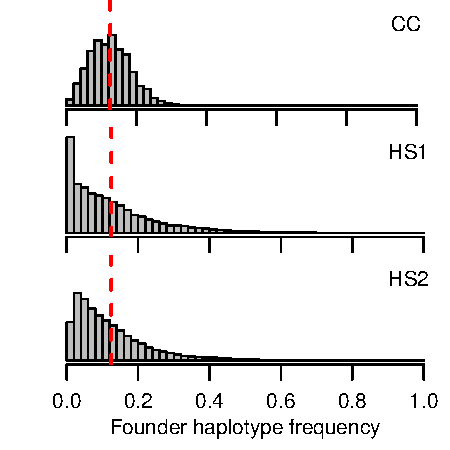
\includegraphics[width=0.7\textwidth, clip, trim={0.3in 0 0 0.1in}]{figures/4-mi/population_allele_freq.pdf}
\caption[Founder haplotype allele frequencies in experimental populations]{Histograms of founder haplotype allele frequencies of loci across the genome for the CC, HS1 and HS2 populations. The vertical dashed red line represents an allele frequency of $1/8$, which would be the mean allele frequency of a perfectly balanced MPP with eight founders. The CC have nicely balanced allele frequencies across the genome, whereas, as expected from rotational breeding, the HS populations have more imbalances, particularly in HS1. These frequencies are based on allele dosages, thus incorporating uncertainty into their estimates.\label{fig:population_freq}}
\end{figure}

\section{Discussion}

In the context of standard and generalizable regression-based QTL mapping in MPP, our multiple imputation approach provides an intuitive approach to incorporate genetic state uncertainty. Theses patterns of uncertainty could present in different ways, and is a more likely issue in MPP where $K$, the number of genetic states, becomes large, particularly in comparison to SNP association ($K=3$). With higher $K$ and certain breeding designs, it becomes more likely that founder haplotype alleles will not be observed at a locus; however, some probability mass is likely still attributed to the founder allele that has been lost because the genetic states are being inferred. This results in the situation highlighted in \textbf{Figure \ref{fig:Leah_example}F} in which near-zero probabilities induce an artificial association. In addition to MI, we considered other approaches to counter spurious associations, but also more powerfully map in these populations than may be possible with standard haplotype-based association.

\begin{figure}
\renewcommand{\familydefault}{\sfdefault}\normalfont
\centering
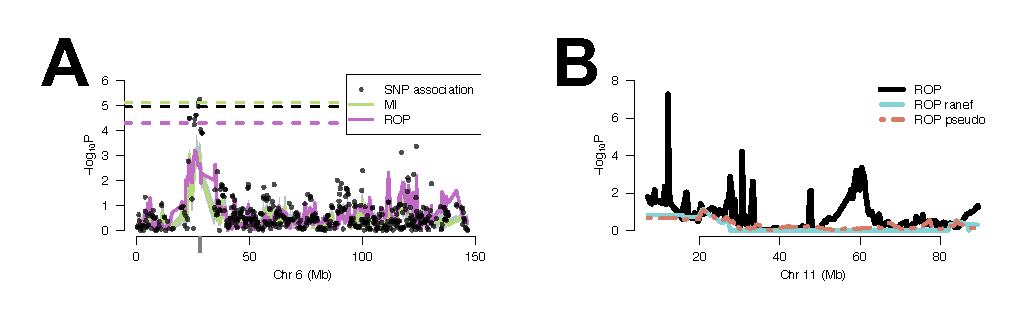
\includegraphics[width=\textwidth]{figures/4-mi/ROP_alternatives.pdf}
\caption[Alternatives to fixef ROP and fixef MI]{Alternative approaches to ROP fixef haplotype association in HS1. Chromosome 6 scans in HS1 of retroperitoneal fatpad mass (A). ROP, MI, and SNP association are included. Although the there is an increased association signal in the haplotype-based methods, the estimation of extra haplotype parameters results in a statistical burden and the associations do not rise above statistical significance. At this locus, one founder possesses a unique SNP allele, and along with the collapsing of the other founders into the other SNP allele, a strong signal is detected. Note the band around the MI association line, which is the 95\% confidence interval on the median p-value across imputations. If the founder haplotype alleles can be captured in a model with less parameters, an increase in power is expected. Comparisons of ROP with the QTL effect fit as a fixed effect with ROP procedures that use shrinkage approaches, either by fitting the QTL as a random effect with a corresponding variance component or through null pseudo-observations, cumulatively weighted to be a single data point (B). Both shrinkage approaches remove the sharp association seen in standard ROP by harshly down-weighting the signal from the near-zero probabilities of the founder B allele (\textbf{Figure \ref{fig:Leah_example}F}).\label{fig:ROP_alternatives}}
\end{figure}

\subsection{SNP association as an alternative to ROP}

One potential alternative to haplotype-based association is SNP association, which is similar to what is commonly used in human GWAS. The founder allele imbalance seen across the genome in HS1 (\textbf{Figure \ref{fig:population_freq}}), as well as the pattern of uncertainty exhibited in \textbf{Figure \ref{fig:Leah_example}F}, in which allele B is not observed, F is very rarely observed, and D, G, and H are poorly distinguishable, exemplify a population that is extremely problematic for ROP, or any form of haplotype association. These problems can be greatly reduced through a simpler genetic model with less genetic states, as in SNP association.  
In effect, a SNP genetic model implicitly reduces the number of genetic states $K$ at a locus, reducing the number of alleles from the $J$ founders to two in a bi-allelic SNP, making it unlikely that an allele is unobserved or very rare. ROP-like SNP-based procedures, as described earlier, could be used, and thus not requiring the additional computational burden of multiple imputation. In MPP with poor founder haplotype reconstructions, SNP association may have greater statistical efficiency compared to MI, whereas ROP would be prone to spurious associations. \textbf{Figure \ref{fig:ROP_alternatives}A} presents a case in HS1 in which SNP association was found to be more powerful for detecting a QTL \citep{Keele2017}. We do not suggest that SNP association is superior for QTL mapping in MPP, but that in situations where founder haplotypes are imbalanced and reconstruction problematic, SNP association can provide a simplified genetic model and avoid spurious associations from ROP. Conversely, SNP association will be less powerful for detecting associations that track with a specific founder haplotype, potentially do to local epistatic interaction, and thus does strongly correlate with a genotyped variant.

\subsection{Shrinkage as an alternative to ROP fixef}

Shrinkage presents a particularly attractive statistically-oriented approach for dealing with issues that result in MPP due to unbalanced founder haplotype frequencies. Rather than fitting an allele parameter wholly-based on very few observations (or even near-zero probabilities), information is shared across genetic states, resulting in predictors of the allele effects that are shrunk toward the overall mean, with more shrinkage present in poorly represented allele, and ultimately resulting in a more conservative modeling approach. This borrowing of information is accomplished by specifying a variance component on the QTL effect; consider the QTL term in the regression model: $\text{QTL}_{i} = \bx_{i}^{\text{T}}\bbetaqtl$, then $\bbetaqtl \sim \text{N}(\mathbf{0}, \bI\tausq)$. Rather than the more conventional fixed effect test of $H_{A}: \bbetaqtl \neq \mathbf{0}$, the variance component can be tested, $H_{A}: \tausq \neq 0$ \citep{Wei2016}. This approach was also included in the analyses of simulated data (as seen in \textbf{Figures \ref{fig:sim_truth}, \ref{fig:sim_scans_dirichlet}, \ref{fig:sim_scans_dilution}, \ref{fig:multi_pval_count1_qtl}, \ref{fig:multi_pval_count1_null}, \ref{fig:multi_pval_dilution_qtl}, \ref{fig:multi_pval_dilution_null}}).

A random effect fitting of the QTL term presents computational challenges compared to fixed effects model, due to need to optimize the likelihood with respect to multiple variance components. This approach could become unfeasible in large samples, particularly in terms of determining significance thresholds through permutations or null bootstraps.

An approximate approach to shrinkage is to include pseudo-observations in the data set. These observations $\tilde{\by}$ represent expectations from $H_{0}$, the model of no QTL effect. Generally $\tilde{\by}$ will contain between $K$ and $j$ elements, depending on the model being fit. Furthermore, these pseudo-observations can be given fractional weights, allowing for the cumulative amount of null pseudo-data to be less than the number of elements of $\tilde{\by}$.

The pseudo-data approach to shrinkage can be made as computationally efficient as standard ROP, making large data sets and computationally expensive procedures like permutations feasible. An unappealing feature of the approach is that selecting the portion of null data to add is arbitrary. In addition, drawing null observations from $H_{0}$ can be done with varying degrees of sophistication, and becomes more complicated with increasingly complex models, such as when covariates are included and a random effect is used to model a polygenic term. Both approaches to shrinkage completely remove the sharp association observed on chromosome 11 for the HS1 rats (\textbf{Figure \ref{fig:ROP_alternatives}B}).

\subsection{Disparity between ROP in simulated and real data}

Based on the simulated data with Dirichlet sampling, ROP performs as well as IM, and is also computationally more efficient and generalizable to other populations. In part we chose simulations of a balanced population like the CC to allow for a greater number of methods to be easily compared with ROP and MI, in particular IM and complete WLS. Our findings suggest that ROP performs well when the data are well-balanced and the genetic state is well-behaved, as with probability dilution; however, deviations from such a setting can result in the inflated associations, which will be pervasive in certain populations (HS1) and still present to a lesser degree in realized balanced populations (CC). As such, MI provides a mapping approach that can restrict these inflated association scores in real data.

\subsection{Summary}

We propose a multiple imputation linear regression procedure for QTL mapping in MPP that accounts for uncertainty in genetic state, which in practice protects against detection of spurious signals caused by unexpected correlations between the phenotype and near-zero allele probabilities or dosages. Our method is flexible to many modeling features, such as population structure modeled as polygenic effect with a corresponding variance component, which is an important consideration in many MPP. The procedure as currently specified uses a single locus model and can easily be used for data being analyzed through ROP, commonly done within software such as the R packages DOQTL \citep{Gatti2014} and qtl2 \citep{Broman2017}. Its computation scales with ROP linearly in terms of the number of imputations performed.

We found the standard ROP approach performed exceptionally well in simulated data, both simulated through probability dilution and Dirichlet sampling, and generally failed to capture or reflect the pattern of associations seen in many of the real data sets we analyzed. This led us to realize that the probability space of the genetic state in MPP is particularly large and complex. Although ROP performs well as a computationally efficient and stable approximation of uncertainty-aware statistical procedures like interval mapping, it clearly struggles with faced with particularly problematic patterns of uncertainty that are also challenging to reliably simulate in practice. Our simulations reveal that the MI procedure is conservative compared to ROP, particularly as uncertainty in genetic state increases. However, we find an alternative conservative procedure preferable when in real data the standard is producing clearly artificial associations.

We have proposed multiple approaches to limiting false positives that result from founder allele frequency imbalances and haplotype uncertainty in MPP, describing a multiple imputations procedure in great detail. MI is easily understood as well as implement, and also flexible to many modeling considerations (alternative models of genetic state, covariates, polygenic term, etc.). Our multiple imputation approach can also incorporate shrinkage methods through a formal random effect fitting of the QTL, which is computationally intensive, and through specification of pseudo-observations. These described approaches provide options for addressing the problems that result from founder haplotype allele frequency imbalances, which can be further compounded though haplotype uncertainty. Though the burden of haplotype uncertainty should lessen as sequencing technologies improve, become less expensive, and are even more extensively used, founder alleles imbalances can still occur in MPP due to genetic drift, certain breeding schemes, and small sample sizes. Methods such as we describe here will be important for reducing the number of false positive associations that are reported, and ultimately feed negative narratives about genetic association studies producing findings that do not replicate.

\newpage

\section{Additional Figures}

\begin{figure}[h!]
\renewcommand{\familydefault}{\sfdefault}\normalfont
\centering
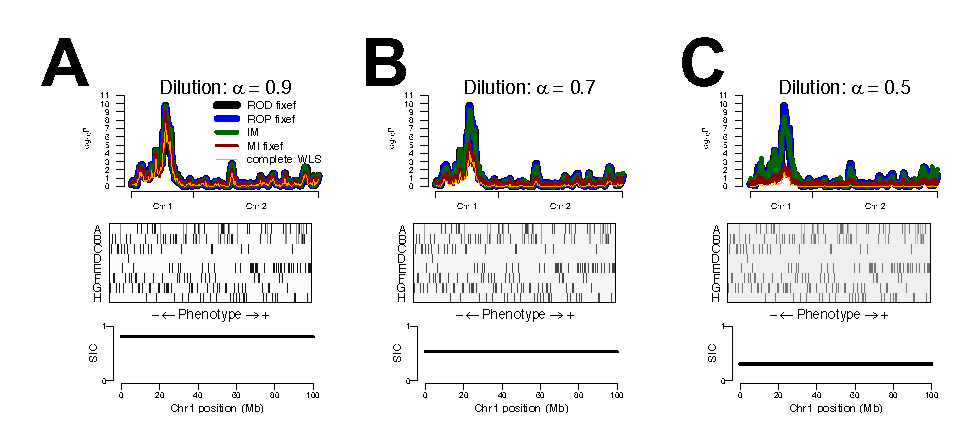
\includegraphics[width=\textwidth, clip, trim={0in 0in 0in 0in}]{figures/4-mi/fixef_mapping_uncertainty_dilution.pdf}
\caption[Effect of uncertainty modeled through probability dilution on genome scan in a single simulated CC-like RI panel]{Comparison of mapping approaches with varying levels of Uncertainty in genetic state simulated through probability dilution with $\alpha = 0.9$ (A), $\alpha = 0.7$ (B), and $\alpha = 0.5$ (C) in 200 simulated CC-like RI strains with a QTL that explains 10\% of phenotypic variation on chromosome 1. Probability dilution is deterministic, with $\alpha$ representing the probability placed on the true genetic state and the remaining mass being evenly allocated to the remaining genetic state categories. The top panel for each subfigure is the genome scan comparing four mapping procedures as well ROD. The middle plot of each subfigure depicts the simulated uncertainty at the QTL for the three scenarios. The bottom plot of each subfigure is the the SIC across chromosome 1, which is summary of information content.\label{fig:sim_scans_dilution}}
\end{figure}

\begin{figure}
\centering
\renewcommand{\familydefault}{\sfdefault}\normalfont
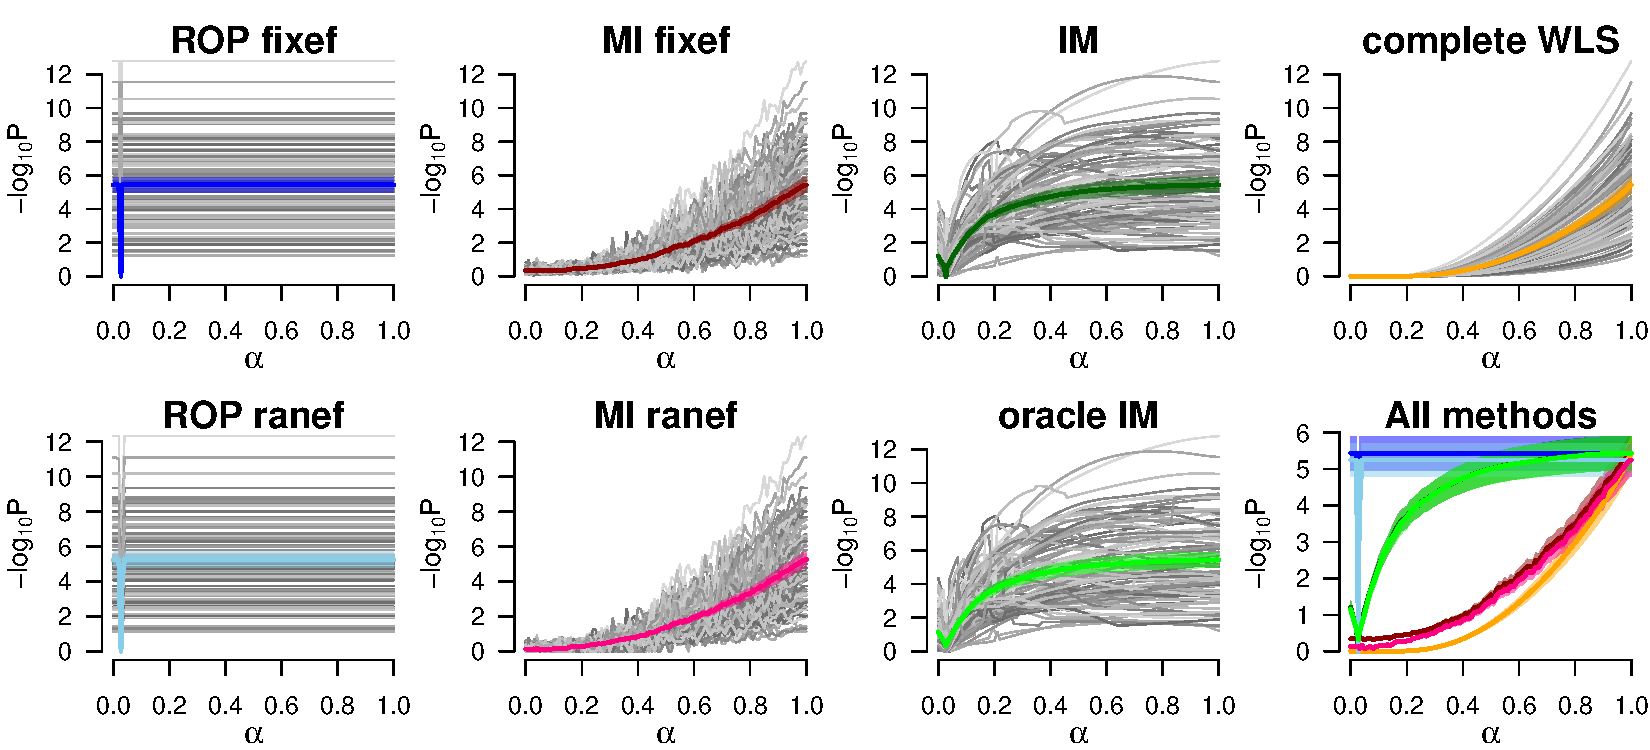
\includegraphics[width=\textwidth]{figures/4-mi/CC_pvalue_fluct_qtl_mean_dilution.pdf}
\caption[Effect of uncertainty modeled through probability dilution sampling on association at QTL in simulated data]{The change in association at 10\% QTL with varying levels of uncertainty, simulated through probability dilution. $\alpha$ is the probability mass of the true genetic state, with the remaining probability mass being split evenly across the other genetic states. Colored lines and transparent bands represent the mean p-value and 95\% confidence interval on the mean p-value for the various mapping procedures (\textbf{Table \ref{tab:mapping_procedures}}) over the 100 populations. Gray lines represent the $-\log_{10}\text{P}$ for a single population.\label{fig:multi_pval_dilution_qtl}}
\end{figure}

\begin{figure}
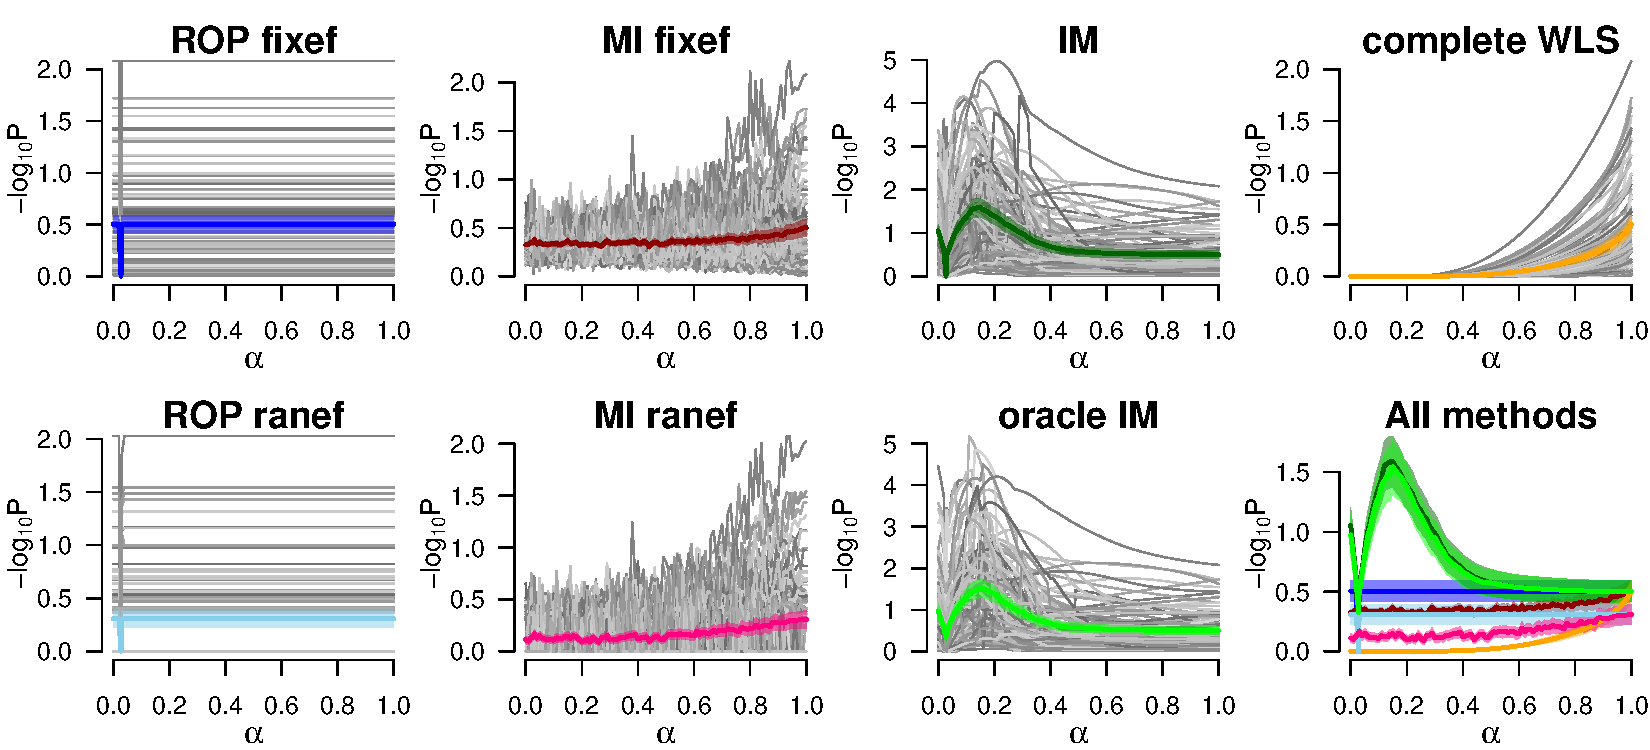
\includegraphics[width=\textwidth]{figures/4-mi/CC_pvalue_fluct_null_mean_dilution.pdf}
\caption[Effect of uncertainty modeled through probability dilution sampling on association at null locus in simulated data]{The change in association at a null locus with varying levels of uncertainty, simulated through probability dilution. $\alpha$ is the probability mass of the true genetic state, with the remaining probability mass being split evenly across the other genetic states. Colored lines and transparent bands represent the mean p-value and 95\% confidence interval on the mean p-value for the various mapping procedures (\textbf{Table \ref{tab:mapping_procedures}}) over the 100 populations. Gray lines represent the $-\log_{10}\text{P}$ for a single population.\label{fig:multi_pval_dilution_null}}
\end{figure}



